% Created 2024-07-08 Mon 22:16
% Intended LaTeX compiler: pdflatex
\documentclass[11pt]{article}
\usepackage[utf8]{inputenc}
\usepackage[T1]{fontenc}
\usepackage{caladea}
\usepackage{graphicx}
\usepackage{longtable}
\usepackage{wrapfig}
\usepackage{rotating}
\usepackage[normalem]{ulem}
\usepackage{amsmath}
\usepackage{amssymb}
\usepackage{capt-of}
\usepackage{hyperref}
\usepackage{fancyhdr}
\title{Novena à Santa Catarina de Labouré}
 \hypersetup{
  pdfauthor={},
  pdftitle={Novena a/à SANTO_NOME},
  pdfkeywords={},
  pdfsubject={},
  pdfcreator={Emacs 29.4 (Org mode 9.6.15)}, 
  pdflang={English}
 }

\title{
  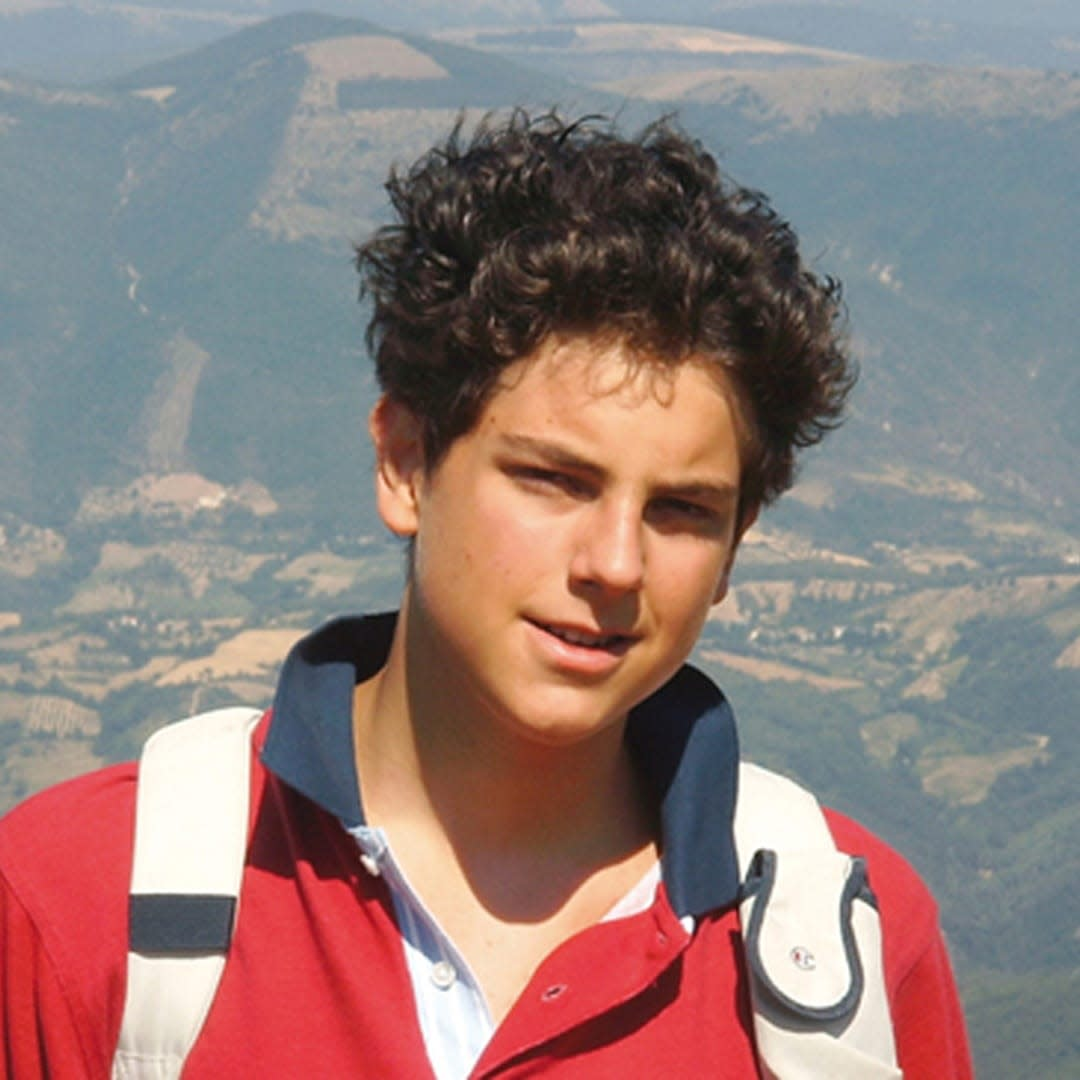
\includegraphics[scale=0.5]{./assets/imagem.jpg} \par
  NOVENA À SANTA CATARINA DE LABOURÉ
}
\author{Garamog, Nina Freitas}
\date{Início da Novena: 19/11 - Data Litúrgica: 27/11}

\begin{document}


\maketitle

\pagestyle{fancy}
  
\centering

\vfill

% configuração do sumário
\renewcommand{\contentsname}{Sumário}
\tableofcontents

\newpage

\section{Orações}
\subsection{Oração Inicial}

Ó Santa Catarina Labouré, que na Sexta Feira da Paixão entrastes em uma casa e encontrastes cinco mil homens bravos como leões, e com vossa santa palavra, abrandastes o coração de todos. Abrandai o coração de meus inimigos. Se tiverem olhos que não me enxerguem, se tiverem ouvidos que não me escutem, se tiverem pernas que não me sigam, se tiverem mãos que não me toquem. Vós que ouvistes dos lábios da Virgem Imaculada que o perigo será grande, tudo parecerá perdido, mas que ela estará convosco, alcançai-me de Deus, a vossa proteção, e a graça que eu vos peço nessa novena. Amém.

\textbf{(Faça aqui seu pedido)}

\textbf{Pai-Nosso, Ave-Maria, Glória}

\subsection{Oração Final} Imploramos ó Deus a vossa misericórdia pela intercessão da bem-aventurada Santa Catarina Labouré, virgem e religiosa, que vos foi agradável pelo serviço da caridade aos pobres e pela propagação da Medalha Milagrosa de Maria Imaculada Mãe do vosso Filho que convosco vive e reina na unidade do Espírito Santo. Por todos os séculos dos séculos. Amém.

Santa Catarina Labouré, rogai por nós.
\vfill 
Créditos: \href{https://www.youtube.com/watch?v=tww2pqasMts&list=PLRL6i6PPLb58c4v96NNGMqFffrI8hSo1H}{Virtude Plena}
\end{document}
